\message{ !name(mainfile.tex)}\documentclass[a4,danish]{article}
\documentclass[11pt,a4paper,twoside,openany,final]{memoir}
\usepackage[utf8]{inputenc}
\usepackage[twoside]{geometry}
%\usepackage[T1]{fontenc}
\usepackage[english]{babel}
\usepackage{amsmath}
\usepackage{amsfonts}
\usepackage{amsthm}
\usepackage[usenames,dvipsnames]{xcolor}
\usepackage{tikz}
\usepackage{amssymb}
\usepackage{graphicx}
\usepackage{flexisym}
\usepackage{hyperref}
\usepackage{xr}
\usepackage[all]{xy}
\usepackage{tikz-cd}
\usepackage{tkz-graph} % To make graphs
\usetikzlibrary{arrows}
\usepackage{tkz-tab}
\usepackage{hyperref}
\usepackage[style=authoryear,backend=bibtex,natbib]{biblatex}
\usepackage{filecontents}
\usepackage[english, status=draft]{fixme}
\fxusetheme{color}
\usepackage{cleveref} 
\usepackage[backgroundcolor=cyan]{todonotes}
\usepackage{wallpaper}
\usepackage{faktor}
\usepackage{nicefrac}
%\usepackage{txfonts}
\usepackage{afterpage} %Til at kunne indsætte tomme sider
\usepackage{pgfplots} %Til at kunne lave grafer
\usepackage{emptypage} %Fjerner sidetal og sidehoveder på tomme sider
\usepackage{multirow}
\usepackage{listings} % To use R language
\lstset{literate=%
{æ}{{\ae}}1
{å}{{\aa}}1
{ø}{{\o}}1
{Æ}{{\AE}}1
{Å}{{\AA}}1
{Ø}{{\O}}1
}
\lstset{ 
  language=R,                     % the language of the code
  basicstyle=\footnotesize\ttfamily, % the size of the fonts that are used for the code
  numberstyle=\tiny\color{blue},  % the style that is used for the line-numbers
  stepnumber=1,                   % the step between two line-numbers. If it is 1, each linewill be numbered
  numbersep=5pt,                  % how far the line-numbers are from the code
  backgroundcolor=\color{white},  % choose the background color. You must add \usepackage{color}
  showspaces=false,               % show spaces adding particular underscores
  showstringspaces=false,         % underline spaces within strings
  showtabs=false,                 % show tabs within strings adding particular underscores
%  frame=single,                   % adds a frame around the code
  rulecolor=\color{black},        % if not set, the frame-color may be changed on line-breaks within not-black text (e.g. commens (green here))
  tabsize=2,                      % sets default tabsize to 2 spaces
  captionpos=b,                   % sets the caption-position to bottom
  breaklines=true,                % sets automatic line breaking
  breakatwhitespace=false,        % sets if automatic breaks should only happen at whitespace
  keywordstyle=\color{RoyalBlue},      % keyword style
  commentstyle=\color{ForestGreen},   % comment style
  xleftmargin=0.5cm,
  xrightmargin=0.5cm
}


%\DisemulatePackage{setspace} START ALTERNATIV SPACING + MARGIN %
%\usepackage{setspace} %
%\doublespacing %
%\setlrmarginsandblock{5cm}{3cm}{*}
%\setulmarginsandblock{2.5cm}{2.5cm}{*}
%\checkandfixthelayout SLUT ALTERNATIV SPACING + MARGIN

\pgfplotsset{width=10cm,compat=1.9}

\begin{filecontents}{bibtest.bib}
@book{Clarke,
  title={Functional Analysis, Calculus of Variations and Optimal Control},
  author={Francis Clarke},
  volume={1},
  year={2013},
  publisher={Springer-Verlag London}
}
@book{Hansen,
  title={Measure Theory},
  author={Ernst Hansen},
  volume={4},
  year={2009},
  publisher={Department of Mathematical Sciences, University of Copenhagen}
}
@article{Topsoee,
  title={Compactness in spaces of measures},
  author={Flemming Topsøe},
  journal={Studia Mathematica},
  volume={36},
  number={3},
  year={1970},
  pages={195--212}
}
@book{Topsoee2,
  title={Topology and measure},
  author={Flemming Topsøe},
  volume={1},
  year={1970},
  publisher={Springer-Verlag, Berlin}
}
@article{Strassen,
  title={The existence of probability measures with given marginals},
  author={Strassen, Volker},
  journal={The Annals of Mathematical Statistics},
  volume={36},
  number={2},
  year={1965},
  pages={423--439}
}
@book{Hoffmann,
  title={Probability in Banach space},
  author={Jørgen Hoffmann-Jørgensen},
  volume={},
  year={1977},
  publisher={Springer}
}
@book{Rudin,
  title={Real and complex analysis},
  author={Walter Rudin},
  volume={3},
  year={1987},
  publisher={McGraw-Hill, Inc.}
}
@book{Rudin2,
  title={Functional analysis},
  author={Walter Rudin},
  volume={2},
  year={1991},
  publisher={McGraw-Hill, Inc.}
}
@book{Aliprantis,
  title={Infinite Dimensional Analysis: A Hitchhiker's Guide},
  author={Charalambos D. Aliprantis and Kim C. Border},
  volume={3},
  year={2006},
  publisher={Springer-Verlag Berlin}
}
@article{Lindvall,
  title={On Strassen's Theorem on stochastic domination},
  author={Torgny Lindvall},
  journal={Electronic Communications in Probability},
  volume={4},
  number={7},
  year={1999},
  pages={51--59}
}
@book{Billingsley,
  title={Convergence of Probability Measures},
  author={Patrick Billingsley},
  volume={2},
  year={2013},
  publisher={John Wiley and Sons}
}
@article{Kamae,
  title={Stochastic inequalities on partially ordered spaces},
  author={Teturo Kamae and Ulrich Krengel and George L. O'Brien},
  journal={The Annals of Probability},
  volume={5},
  number={6},
  year={1977},
  pages={899--912}
}
@book{Sokol,
  title={Advanced Probability},
  author={Alexander Sokol and Anders Rønn-Nielsen},
  volume={4},
  year={2016},
  publisher={Department of Mathematical Sciences, University of Copenhagen}
}
@book{Bladt,
  title={Matrix–exponential distributions in Applied Probability},
  author={Mogens Bladt and Bo Friis Nielsen},
  volume={1},
  year={2017},
  publisher={Springer (Pending)}
}
@article{Rosenblum,
  title={Simple Examples of Estimating Causal Effects Using Targeted Maximum Likelihood Estimation},
  author={Michael Rosenblum and Mark J. van der Laan},
  journal={U.C. Berkeley Division of Biostatistics Working Paper Series},
  volume={Working Paper 262},
  year={2010}
}
@Inbook{Kennedy,
author="Kennedy, Edward H.",
editor="He, Hua
and Wu, Pan
and Chen, Ding-Geng (Din)",
title="Semiparametric Theory and Empirical Processes in Causal Inference",
bookTitle="Statistical Causal Inferences and Their Applications in Public Health Research",
year="2016",
publisher="Springer International Publishing",
address="Cham",
pages="141--167",
isbn="978-3-319-41259-7",
doi="10.1007/978-3-319-41259-7_8",
url="https://doi.org/10.1007/978-3-319-41259-7_8"
}
@book{TargetedLearning,
  title={Targeted Learning in Data Science},
  author={Mark J. van der Laan and Sherri Rose},
  volume={1},
  year={2011},
  publisher={Springer}
}
@article{Wikkelsoee,
  title={Prediction of postpartum blood transfusion -- risk factors and recurrence.},
  author={AJ Wikkelsøe and S Hjortøe and TA Gerds and AM Møller and J Langhoff-Roos}, 
  journal={The journal of maternal-fetal and neonatal medicine},
  volume={27},
  number={16},
  year={2014}
}
@book{Causality,
  title={Elements of causal inference},
  author={Jonas Peters and Dominik Janzing and Bernhard Schölkopf},
  volume={1},
  year={2017},
  publisher={MIT Press}
}
@book{Asymptotic,
  title={Asymptotic Statistics},
  author={A. W. Van der Vaart},
  volume={3},
  year={2000},
  publisher={Cambridge University Press}
}
@article{PPHcause,
  title={Recent Advances in the Management of Major Postpartum Haemorrhage - A Review},
  author={P Reddi Rani1 and Jasmina Begum}, 
  journal={Journal of Clinical and Diagnostic Research},
  volume={11},
  number={2},
  year={2017}
}
@Manual{SuperLearner,
    title = {SuperLearner: Super Learner Prediction},
    author = {Eric Polley and Erin LeDell and Chris Kennedy and Mark {van der Laan}},
    year = {2018},
    note = {R package version 2.0-23},
    url = {https://CRAN.R-project.org/package=SuperLearner}
}
@Article{tmle,
    title = {{tmle}: An {R} Package for  Targeted Maximum Likelihood Estimation},
    author = {Susan Gruber and Mark J. {van der Laan}},
    journal = {Journal of Statistical Software},
    year = {2012},
    volume = {51},
    number = {13},
    pages = {1--35},
    url = {http://www.jstatsoft.org/v51/i13/},
}



\end{filecontents}

\addbibresource{bibtest.bib}


\chapterstyle{verville}


\setlength{\parindent}{0em}
\setlength{\parskip}{1em}
\renewcommand{\baselinestretch}{1}


\DeclareMathOperator{\supp}{supp}
\DeclareMathOperator{\Ext}{Ext}
\DeclareMathOperator{\Aut}{Aut}
\DeclareMathOperator{\Ran}{Ran}
\DeclareMathOperator{\Prob}{Prob}
\DeclareMathOperator{\conv}{conv}
\DeclareMathOperator{\AR}{AR}
\DeclareMathOperator{\Homeo}{Homeo}

\makepagestyle{abs}
    \makeevenhead{abs}{}{}{}
    \makeoddhead{abs}{}{}{}
    \makeevenfoot{abs}{}{\scshape I }{}
    \makeoddfoot{abs}{}{\scshape  I }{}
    %\makeheadrule{abs}{\textwidth}{\normalrulethickness}
    %\makefootrule{abs}{\textwidth}{\normalrulethickness}{\footruleskip}
\pagestyle{abs}


\makepagestyle{cont}
    \makeevenhead{cont}{}{}{}
    \makeoddhead{cont}{}{}{}
    \makeevenfoot{cont}{}{\scshape II }{}
    \makeoddfoot{cont}{}{\scshape  II }{}
    %\makeheadrule{abs}{\textwidth}{\normalrulethickness}
    %\makefootrule{abs}{\textwidth}{\normalrulethickness}{\footruleskip}
\pagestyle{cont}

\newcommand{\lv}{\lVert}
\newcommand{\rv}{\rVert}


\renewcommand\chaptermarksn[1]{}
\nouppercaseheads
\createmark{chapter}{left}{shownumber}{}{.\space}
\makepagestyle{dut}
    \makeevenhead{dut}{\scshape\rightmark}{}{}
    \makeoddhead{dut}{\scshape\leftmark}{}{}
    \makeevenfoot{dut}{}{\scshape $-$ \thepage\ $-$}{}
    \makeoddfoot{dut}{}{\scshape $-$ \thepage\ $-$}{}
    \makeheadrule{dut}{\textwidth}{\normalrulethickness}
    \makefootrule{dut}{\textwidth}{\normalrulethickness}{\footruleskip}
\pagestyle{dut}

\makepagestyle{chap}
    \makeevenhead{chap}{}{}{}
    \makeoddhead{chap}{}{}{}
    \makeevenfoot{chap}{}{\scshape $-$ \thepage\ $-$}{}
    \makeoddfoot{chap}{}{\scshape $-$ \thepage\ $-$}{}
    \makefootrule{chap}{\textwidth}{\normalrulethickness}{\footruleskip}
\copypagestyle{plain}{chap}

\newcommand{\R}{\mathbb{R}}
\newcommand{\C}{\mathbb{C}}
\newcommand{\N}{\mathbb{N}}
\newcommand{\E}{\mathrm{E}}
\newcommand{\Var}{\mathrm{Var}}
\newcommand{\mbr}{(X,\mathcal{A})}
\newcommand{\Z}{\mathbb{Z}}
\newcommand{\Q}{\mathbb{Q}}
\newcommand{\F}{\mathcal{F}}
\newcommand{\A}{\mathcal{A}}
\newcommand{\cc}{C_c}
\newcommand{\PP}{\mathcal{P}}
\newcommand{\B}{\mathcal{B}}
\newcommand{\ee}{\epsilon}
\newcommand{\la}{\lambda}
\renewcommand{\H}{\mathcal{H}}
\newcommand{\pp}{\text{Prob}}
\newcommand{\U}{\mathcal{U}}
\newcommand{\dd}{\mathrm{d}}

\newcommand{\nocontentsline}[3]{}
\newcommand{\tocless}[2]{\bgroup\let\addcontentsline=\nocontentsline#1{#2}\egroup} % Fjern sections fra Table of Contents

\makeatletter
\newcommand{\Spvek}[2][r]{%
  \gdef\@VORNE{1}
  \left(\hskip-\arraycolsep%
    \begin{array}{#1}\vekSp@lten{#2}\end{array}%
  \hskip-\arraycolsep\right)}

\def\vekSp@lten#1{\xvekSp@lten#1;vekL@stLine;}
\def\vekL@stLine{vekL@stLine}
\def\xvekSp@lten#1;{\def\temp{#1}%
  \ifx\temp\vekL@stLine
  \else
    \ifnum\@VORNE=1\gdef\@VORNE{0}
    \else\@arraycr\fi%
    #1%
    \expandafter\xvekSp@lten
  \fi}
\makeatother

\def\acts{\curvearrowright}

\newcommand{\K}{\mathbb{K}}

\newtheoremstyle{break}
	{\topsep}{\topsep}
	{\bfseries}{}
	{\newline}{}
\theoremstyle{break}
\newtheorem{theorem}[subsection]{Theorem}
\newtheorem{lemma}[subsection]{Lemma}
\newtheorem{proposition}[subsection]{Proposition}
\newtheorem{corollary}[subsection]{Corollary}
\newtheorem{definition}[subsection]{Definition}
\newtheoremstyle{Break}
	{\topsep}{\topsep}
	{}{}
	{\bfseries}{}
	{\newline}{}
\theoremstyle{Break}
\newtheorem{example}[subsection]{Example}
\newtheorem{remark}[subsection]{Remark}
\newtheorem{note}[subsection]{Note}
\setcounter{secnumdepth}{0}
\usepackage{xpatch}
\xpatchcmd{\proof}{\ignorespaces}{\mbox{}\\\ignorespaces}{}{}

\newcommand*{\diff}{\mathop{}\!\mathrm{d}}

\newcommand\blankpage{%
    \null
    \thispagestyle{empty}%
    \addtocounter{page}{-1}%
    \newpage}
    
\DeclareNameAlias{sortname}{last-first} % Med flere forfattere bliver alle navne på formen
\DeclareNameAlias{default}{last-first} % : "LastName, FirstName MiddleName

\newcommand{\blank}{\makebox[1ex]{\textbf{$\cdot$}}} % Command to placeholder

\newcommand{\indep}{\rotatebox[origin=c]{90}{$\models$}} % Independent symbol

\title{Statistical analysis of shapes}
\author{Mads and Anders}
\date{\today}

%%% Local Variables:
%%% mode: latex
%%% TeX-master: "mainfile"
%%% End:


\begin{document}

\message{ !name(tangent_space_of_curves.tex) !offset(-7) }
\section{The manifold of curves}
\label{sec:manifold-curves}

A 2-dimensional shape can be thought of as a closed (smooth) curve in $\R^2$. Thus, we want to define a manifold structure on the space of these curves. Doing this mathematically correct is rather technical because we need to consider quotient spaces of infinite dimensional manifolds. In our exposition we shall to a large extend ``define our way out of this'' by, for example, defining tangent vectors of curves instead of deducing how these look like from the formal definition of the underlying manifold. We shall motivate our definitons geometrically and then deduce some properties from these definitons -- properties, which can also be deduced from the formal definitions. At the end of this section we briefly address what we miss with our more informal treatment.

A shape in $\R^2$ can either be thought of as a parametrized object, e.g., as a function $\S^1 \ni \theta \mapsto c(\theta) \in \R^2$; but it can also be thought of as an unparametrized object, e.g., the \textit{image} of such a function $\text{Im}(c) \subset \R^2$ (as illustrated in Figure~\ref{fig:circle-mapping}). We impose some smoothness structure on the curves and define the spaces we want to consider formally as
\begin{equation*}
  \begin{aligned}
    \I & := \I(\S^1, \R^2)  :=  \{ ...? \}, \\
    \mathcal{I} & := \mathcal{I}(\S^1, \R^2)  := \I(\S^1, \R^2)/\mathrm{Diff}(\S^1).
  \end{aligned}
\end{equation*}
$\I$ is the space of \textit{immersion} of the unit circle into $\R^2$, and $\mathcal{I}$ is then this space modulo reparametrization, i.e., we identify two object $q,p \in \I$ in $\mathcal{I}$ if $q=p \circ \phi$, where $\phi \in \mathrm{Diff}(\S^1)$ is a diffeomorphism on the unit circle.

When our interest is upon the \textit{shape}, we are not really interested in the underlying parametrization of this shape, and so we are mostly interested in the space $\mathcal{I}$. However, it is easiest to construct a manifold structure on $\I$ and then deduce one on $\mathcal{I}$, so we start by considering the parametrized space of immersions.

\begin{figure}
  \centerline{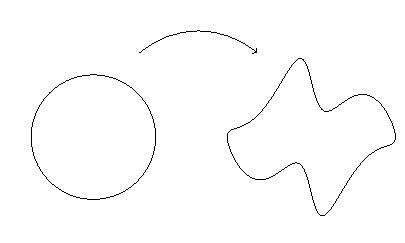
\includegraphics[width=0.9\linewidth]{circle_mapping.pdf}}
  \caption{A simple shape. We can think of a shape as the whole
    mapping, or simply as the subset to the right.}
  \label{fig:circle-mapping}
\end{figure}

\subsection{The manifold of parametrized curves -- $\I(\S^1, \R^2)$}
\label{sec:parametrized-curves}

The first structure we want to impose on our manifold of curves is tangent spaces and tangent vectors to our elements in the space.

For ordinary finite dimensional manifolds $M$ \hl{we have so far worked with} the definition of tangents vectors as \textit{derivatives}. This is a rather abstract construction, which, however, turns out to be nice to work with. Fortunalety, we know that this definition corresponds to the more geometrically intuitive definition of tangent vectors at a point $m \in M$ as derivatives of paths going through $m$. We shall use this a motivation for our definition of tangent vectors to points in $\I$.

Consider a point $c\in \I$ and a path in $\I$ defined around $0$ that goes through the point $c$. This path is a map
\begin{equation}
  \label{eq:path-in-imm}
  [-\epsilon, \epsilon] \ni t \mapsto  q(t, \blank) :=  (\theta\mapsto q(t, \theta)) \in \I,
  \quad q(0,\theta) = c(\theta),
\end{equation}
i.e., for each $t$ we get a parametrized curve, and at 0 we get the curve $c$. We can also think of this a (smooth) map
\begin{equation*}
  [-\epsilon, \epsilon] \times \S^1  \ni (t, \theta) \mapsto q(t, \theta) \in \R^2.
\end{equation*}
As in the finite dimensional case we can now take the \textit{time derivate} of our path and evaluate this at 0; of course, this is technically not obvious, as our constructed path maps into a function space, but we shall here simply take this derivative to be understood pointwise:

\begin{definition}
  The tangent space $T_{c}\I$ to an element $c \in \I$ consists of all function
  $h\colon \S^1 \rightarrow \R^2$ such that
  \begin{equation*}
    h(\theta) = q_t(0, \theta) := \frac{\partial }{\partial t} \bigg\vert_{t=0} q(t,\theta),
  \end{equation*}
  where $q$ is some path passing through $c$ at 0 (as defined in \eqref{eq:path-in-imm}).
\end{definition}

By this definition, we can essentially think of tangent vectors in $\I$ as vector fields on the circle. Figure~\ref{fig:def-tang-imm} illustrates the idea behind the definition.

\begin{figure}
  \centering
  \begin{subfigure}{.49\textwidth}
    \centering
    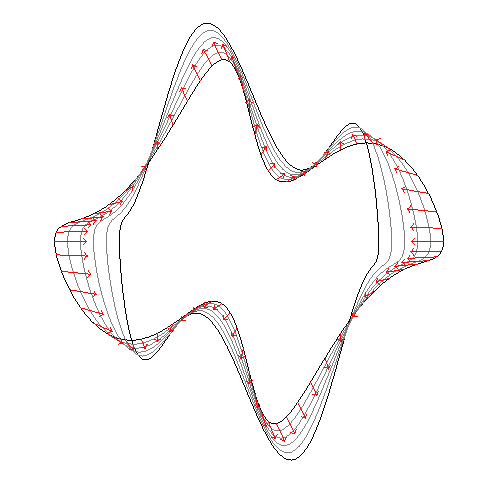
\includegraphics[width=1\linewidth]{path.pdf}
  \end{subfigure}
  \begin{subfigure}{.49\textwidth}
    \centering
    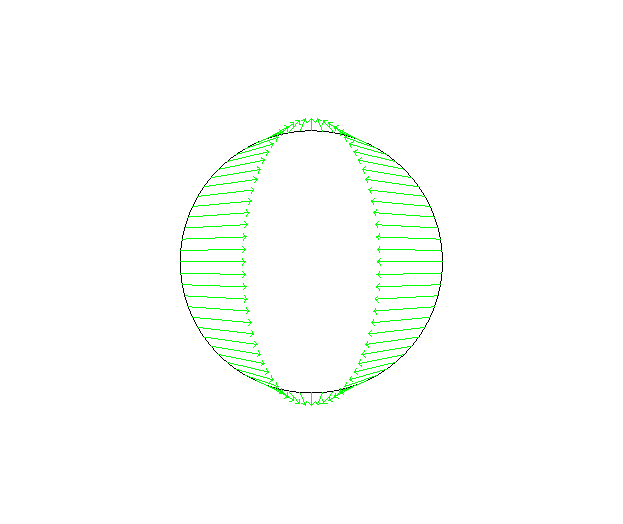
\includegraphics[width=0.8\linewidth]{circle_vectorfield.pdf}
  \end{subfigure}
  \caption{Illustration of tangent vectors in $\I$. The left illustration shows a path in the space of curves and how to obtain a tangent vector from this. The right illustration shows how to think of this tangent vector as a vector field on the circle.}
  \label{fig:def-tang-imm}
\end{figure}

We want to make our space of curves into a Riemmanian manifold so the next step is to impose a metric
\hl{[why do we/others call it a metric -- shouldn't it be an inner product?]}
on the tangent spaces. Because the tangent spaces are function spaces, the most obvious metric to use is some version of the $\mathrm{L}^2$ metric.

\begin{definition}
  The \textit{$\mathrm{G}$ metric} or \textit{$\mathrm{G}_c$ metric} at the point $c \in \I$ is defined as
  \begin{equation*}
    \mathrm{G}_c(h,k) :=
    \left(
      \int_{\S^{1}} \left\langle{h(\theta)
          , k(\theta)}\right\rangle |c_{\theta}| \diff \theta
    \right)^{\frac{1}{2}},
  \end{equation*}
  $h,k \in T_cB = C^{\infty}(\S^1,\R^2)$.
\end{definition}

Adding the parameter derivative $c_{\theta}$ makes the metric invariant to reparametrizations which is essential when we want to let this fall down as a metric on $\mathcal{I}$. From this definition it is straightforward to define a notion of \textit{length} of a path in $\I$ which again allows us to define a \textit{distance} between two point in our space of curves. By defintion, the pointwise time derivative at $t$ of a path $t \mapsto q(t, \blank)$ in $\I$ is a tangent vector to the curve $q(t,\blank)$, so the following definition makes sense.

\begin{definition}
  \label{def:length-in-imm}
  Let $t \mapsto q(t,\blank)$ be a path in $\I$ with $t \in [0,1]$. The \textit{length} of the path $q$ with respect to the $\mathrm{G}$ metric  is
  \begin{equation*}
    L(q) := \int_{0}^{1} \mathrm{G}_{q(t,\blank)}(q_t,q_t) \diff t =
    \int_{0}^{1}
    \left(
      \int_{\S^{1}} \|q_t\|^2 |q_{\theta}| \diff \theta
    \right)^{\frac{1}{2}}
    \diff t.
  \end{equation*}
  The \textit{geodesic distance} \hl{[geodesic?]} between to curves $b,c \in \I$ (with respect to the $\mathrm{G}$ metric) is
  \begin{equation*}
    D(b,c) := \inf_{q \in \mathcal{Q}} L(q),
  \end{equation*}
  where $\mathcal{Q}$ denotes all paths $q$, such that $q(0,\blank)=b$ and $q(1,\blank)=c$.
\end{definition}


\subsection{The manifold of unparametrized curves -- $\mathcal{I}(\S^1, \R^2)$}
\label{sec:manif-unpar-curv}

Using the setup from the previous section, we now define a manifold structure on $\mathcal{I}$. As it is easiest to represent element of this space with element from $\I$, we are particularly interested in how to calculate the length of a path in $\mathcal{I}$ directly from a parametrized representative of this path in $\I$. For a parametrized curve $c \in \I$ we write $\pi(c) := \mathrm{Im}(c)\in \mathcal{I}$ for the projection onto the quotient space, and we refer to $c\in\I$ as a \textit{(parametrized) representative} for $\pi(c) \in \mathcal{I}$. Similarly for a path $q = q(t, \blank) \in \I$ we construct the projection $\pi(q) = \pi(q(t,\blank)) \in \mathcal{I}$ and refer to $q$ as a representative for $\pi(q)$.

First of all we need to know how the tangent vectors of the quotient space $\mathcal{I}$ look like. We cannot directly use the same approach as in the previous subsection, because our definition of tangent vector would then be
sensitive to reparametrizations: Consider a time-dependent
reparametrization $\phi(t,\theta)$, or, equivalently, a path $t \mapsto \phi(t,
\blank)$ in $\text{Diff}(\S^1)$; then the two paths $t \mapsto
\pi(q(t, \blank))$ and $t \mapsto \pi(q(t, \phi(t, \blank)))$ are
identical in $\mathcal{I}$ but give rise to two different vector fields.

To make better sense of the tangents vectors of the quotient space, we
use the following result.

\begin{proposition}
  \label{prop:horizontal-path}
  For every path $t \mapsto q(t, \blank)$ in $\mathrm{Imm}$ there exists a
  time-dependent reparametrization $t \mapsto \phi(t, \blank) \in
  \mathrm{Diff}(\S^{1})$ such that the path
  \begin{equation*}
    t \mapsto \tilde{q}(t, \theta):=q(t, \phi(t,\theta))
  \end{equation*}
  fulfills
  $\langle \tilde{q}_t, \tilde{q}_{\theta}\rangle=0$ for all $(t,\theta) \in [0,1]\times \S^1$, and such that $\phi(0, \theta)=\theta$. Furthermore, it holds that
  \begin{equation}
    \label{eq:canon-repar}
    \phi_t = a \circ \phi
    = -\frac{\langle q_t \circ \phi, q_{\theta} \circ \phi\rangle}{|q_{\theta}\circ \phi|^2},
    \quad a := -\frac{\langle q_t,
      q_{\theta}\rangle}{|q_{\theta}|^2}.
  \end{equation}
\end{proposition}

\begin{proof}
  \hl{todo or ref.}
\end{proof}

\begin{remark}
  \label{remark:ortho-decom}
  \begin{enumerate}
  \item  When we write $\tilde{q}$ in the following, we shall we refer to a path obtained from another path $q$ by reparametrizing with $\phi$ above.
  \item Note that for every vector field $h \in T_c(\I)$, determined from the path $q$, we can make a pointwise decomposition of $h$ onto $q_{\theta}(0, \blank)$ and $iq_{\theta}(0, \blank)$ by using the pointwise orthogonal projection. Explicitly we have that
  \begin{equation*}
    h = q_t = p_{q_{\theta}}(q_{t}) + p_{iq_{\theta}}(q_{t}),
  \end{equation*}
  where $p$ is taken to be the standard \textit{pointwise} $\R^2$ orthogonal projection, which is given as
  \begin{equation*}
    p_v(u) = \frac{\langle v, u \rangle}{|v|^2} v, \quad u, v \in \R^2.
  \end{equation*}
  More correctly we should thus write
  \begin{equation*}
    h(\theta) = q_t(0,\theta) = p_{q_{\theta}(0,\theta)}(q_{t}(0,\theta)) +
    p_{iq_{\theta}(0,\theta)}(q_{t}(0,\theta)).
  \end{equation*}
  From this we see that the time derivative of the reparametrization in the previous Proposition is the coefficient function for the projection onto the parameter derivative of the original path $q$; this becomes relevant in a moment.
\end{enumerate}
\end{remark}

We can use this result to define tangent vectors to elements of $\mathcal{I}$ in
a consistent way:

\begin{definition}
  \label{def:tang-quotient}
  A \textit{tangent vector} $h$ to an element $\pi(c) \in \mathcal{I}$ is defined as a vector fields obtained from some path $(-\epsilon, \epsilon) \ni t \mapsto q(t, \blank) \in \I$, with $q(0,\blank) = c$, by
  \begin{equation}
    \label{eq:tang-quotient}
    h(\theta) = \frac{\partial }{\partial t} \bigg\vert_{t=0} \tilde{q}(t,\theta)
    = \frac{\partial }{\partial t} \bigg\vert_{t=0} q(t, \phi(t,\theta)),
  \end{equation}
  with $\tilde{q}$ and $\phi$ given in accordance with remark~\ref{remark:ortho-decom}.

  \hl{[NB: Does this actually solve the problem about define the ubiquity in defining tangent vectors? Not clear that applying $\phi$ to a reparametrization of $q$ will yield the same result? However, it shows that we can always think of are path as moving orthonormally; but maybe we should compine this definition with the proposition below?]}
\end{definition}

First we note that this gives us the following visualization of the tangents spaces of $B$.

\begin{proposition}
The tangent space to an element $\pi(c) \in \mathcal{I}$ consists of orthonormal vector fields on the circle, i.e.,
  \begin{equation*}
    T_{\pi(c)}(\mathcal{I}) =
    \left\{
      b i c_{\theta} \mid b \in C^{\infty}(\S^1,\R)
    \right\}.
  \end{equation*}
\end{proposition}

\begin{proof}
  This follows from Definition~\ref{def:tang-quotient} and the property of the reparametrization $\phi$.
\end{proof}

As the length of a path in $\mathcal{I}$ is our primary concern, we skip straight to this without actually defining the inner product on the tangent spaces. The central idea is to mimic Definition~\ref{def:length-in-imm} on the reparametrized path $\tilde{q}$; and though we don't bother to go trough a inner product on the tangent spaces, we note that by this construction the time derivative of the path $\tilde{q}$ is a valid tangent vector in $\mathcal{I}$ at every point $\pi(q(t,\blank))$

\begin{definition}
  The \textit{length} in $\mathcal{I}$ of a path $\mathrm{q}=\pi(q)$ is
  \begin{equation*}
    \mathcal{L}(\mathrm{q})= \mathcal{L}(\pi(q)) := L(\tilde{q}) =
    \int_{0}^{1}
    \left(
      \int_{\S^{1}} \|\tilde{q}_t\|^2 |\tilde{q}_{\theta}| \diff \theta
    \right)^{\frac{1}{2}}
    \diff t,
  \end{equation*}
  with $\tilde{q}(t,\theta)=q(t,\phi(\theta))$ as in remark~\ref{remark:ortho-decom}.
  The \textit{geodesic distance} between to shapes $\mathrm{b}, \mathrm{c} \in \mathcal{I}$ represented by $c,b \in \I$, is
  \begin{equation*}
    \mathcal{D}(\mathrm{b},\mathrm{c}) = \mathcal{D}(\pi(b),\pi(c)) := \inf_{q \in \mathrm{Q}} \mathcal{L}(q),
  \end{equation*}
  where $\mathrm{Q}$ denotes all paths $\mathrm{q}$ in $\mathcal{I}$, such that $\mathrm{q}(0)=\pi(b)$ and $\mathrm{q}(1)=\pi(c)$.
\end{definition}

\begin{proposition}
  \label{prop:length-quotient}
    $\mathcal{L}$ is well-defined, and for any representative $t \mapsto q(t, \blank) \in \I $ of the path $t \mapsto \tilde{q}(t) \in B$ the length can be calculated as
    \begin{equation}
      \label{eq:length-quotient}
    \mathcal{L}(\tilde{q}) = \int_{0}^{1}
    \left(
      \int_{\S^1}  \frac{\langle q_t, i q_{\theta}\rangle^2}{|q_{\theta}|} \diff \theta
    \right)^{\frac{1}{2}} \diff t.
  \end{equation}
\end{proposition}

\begin{proof}
  For ease of notation, write $q \circ \phi$ to mean $q(t, \phi(t,\theta))$ and so on during this proof.
  First, we shows that \eqref{eq:length-quotient} implies that $\mathcal{L}$ is well-defined; so assume \eqref{eq:length-quotient} holds and let $q(t,\blank)$ and $p(t, \blank)$ be two different representatives for $\tilde{q}(t)$. This means that we must have a reparametrization $\psi(t,\theta)$ such that
  \begin{equation*}
    p(t, \psi(t,\theta)) = q(t, \theta).
  \end{equation*}
  Then
  \begin{equation*}
    p_t = q_t\circ \psi + \psi_t (q_t \circ \psi), \quad
    p_{\theta} = \psi_{\theta}(q_{\theta} \circ \psi),
  \end{equation*}
  so
  \begin{equation*}
    \begin{aligned}
      \left\langle
        p_t, i p_{\theta}
      \right\rangle
     &  =     \left\langle
        q_t \circ \psi + \psi_t (q_{\theta} \circ \psi),
        \psi_{\theta} (iq_{\theta} \circ \psi)
      \right\rangle \\
     & =     \left\langle
        q_t \circ \psi,
        \psi_{\theta} (iq_{\theta} \circ \psi)
      \right\rangle \\
      & = (\langle q_t, i q_{\theta}\rangle \circ\psi) \psi_{\theta},
    \end{aligned}
  \end{equation*}
  and thus
  \begin{equation*}
    \int_{\S^1} \frac{\langle p_t, i p_{\theta}\rangle^2}{|p_{\theta}|} \diff \theta
    =
    \int_{\S^1}
    \left(
      \frac{\langle q_t, i q_{\theta}\rangle^2}{|q_{\theta}|}
    \right) \circ \psi |\psi_{\theta}| \diff \theta
    =    \int_{\S^1}
      \frac{\langle q_t, i q_{\theta}\rangle^2}{|q_{\theta}|}  \diff \theta,
    \end{equation*}
    which shows that the length does not depend on the parametrization of the path.

  Next, by construction, the tangent vectors along the path $\tilde{q}$ in $B$ is given as
  \begin{equation*}
    \frac{\partial }{\partial t}  (q \circ \phi)
    = q_t \circ \phi + \phi_t (q_{\theta} \circ \phi)
  \end{equation*}
  Now, as in remark~\ref{remark:ortho-decom}, decompose $q_t \circ \phi $ by projecting pointwise onto $q_t \circ \phi $ and $i q_t \circ \phi $. Then we get
  \begin{equation*}
    q_t \circ \phi =
    % \frac{\langle q_t \circ \phi, iq_{\theta} \circ \phi \rangle}
    % {|q_{\theta} \circ \phi|^2}(iq_{\theta} \circ \phi) +
    % \frac{\langle q_t \circ \phi, q_{\theta} \circ \phi \rangle}
    % {|q_{\theta} \circ \phi|^2}(q_{\theta} \circ \phi),
    % =
    \left(
      \frac{\langle q_t  , iq_{\theta}   \rangle}
    {|q_{\theta}  |^2}iq_{\theta}
  \right) \circ \phi +
  \left(
    \frac{\langle q_t  , q_{\theta}   \rangle}
    {|q_{\theta}  |^2}q_{\theta}
  \right) \circ \phi,
  \end{equation*}
  and by Proposition~\ref{prop:horizontal-path} we see that the last term cancels with
  $\phi_t(q_{\theta}\circ \phi)$, so
  \begin{equation*}
    \frac{\partial }{\partial t} ( q \circ \phi )=
    % \frac{\langle q_t \circ \phi, iq_{\theta} \circ \phi \rangle}
    % {|q_{\theta} \circ \phi|^2}(iq_{\theta} \circ \phi)
    % =
    \left(
      \frac{\langle q_t  , iq_{\theta}   \rangle}
      {|q_{\theta}  |^2}iq_{\theta}
    \right)
    \circ \phi.
  \end{equation*}
  For any fixed $t \in [0,1]$, the reparametrization $\phi$ is just an ordinary reparametrization of the curve $\theta \mapsto q(t,\theta)$, so by invariance of the metric we have that
  \begin{equation*}
    \begin{aligned}
    & G_{q(t,\phi(t,\blank))}^2
    \left( \frac{\partial }{\partial t} ( q \circ \phi ),
      \frac{\partial }{\partial t} ( q \circ \phi )
  \right) \\
  & \quad=  G_{q(t,\phi(t,\blank))}^2
    \left(
          \left(
      \frac{\langle q_t  , iq_{\theta}   \rangle}
      {|q_{\theta}  |^2}iq_{\theta}
    \right)
    \circ \phi,
        \left(
      \frac{\langle q_t  , iq_{\theta}   \rangle}
      {|q_{\theta}  |^2}iq_{\theta}
    \right)
    \circ \phi
    \right) \\
    & \quad =
    G_{q(t,\blank)}^2
    \left(
      \frac{\langle q_t  , iq_{\theta}   \rangle}
      {|q_{\theta}  |^2}iq_{\theta} ,
      \frac{\langle q_t  , iq_{\theta}   \rangle}
      {|q_{\theta}  |^2}iq_{\theta}
    \right) \\
    & \quad =
    \int_{\S^1}
    \left\|
      \frac{\langle q_t  , iq_{\theta}   \rangle}
      {|q_{\theta}  |^2}iq_{\theta}
    \right\|^2 |q_{\theta}  | \diff \theta \\
    & \quad =
    \int_{\S^1}
      \frac{\langle q_t  , iq_{\theta}   \rangle^2}
      {|q_{\theta}  |}  \diff \theta,
  \end{aligned}
\end{equation*}
from which \eqref{eq:length-quotient} follows immediately by definition.
\end{proof}

\hl{Some concluding text...}

\subsection{\hl{Comparing this to the formal construction as a Frechet manifold}}
\label{sec:hlcomp-this-form}

\hl{... a lot of references ...}



%%% Local Variables:
%%% mode: latex
%%% TeX-master: "mainfile"
%%% End:

\message{ !name(mainfile.tex) !offset(-355) }

\end{document}
